\section{Durchführung und Aufbau}
\label{sec:Durchführung}
\subsection{Messprogramm für die Ablenkung im E-Feld}
Zu Beginn wird die Empfindlichkeit zwischen der Ablenkspannung $U_\text{d}$ und der Verschiebung $D$ für fünf verschiedene Beschleunigungsspannungen $U_\text{B}$ untersucht. Dazu wird die Schaltung aus Abbildung \eqref{fig:Schaltung1} aufgebaut.

\begin{figure}[H]
  \centering
  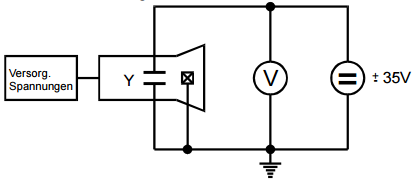
\includegraphics[height=5cm]{picture/Schaltung1}
  \caption{Aufbau zur Messung der Abhängigkeit zwischen der Verschiebung und der Ablenkspannung. \cite[5]{V501}}
  \label{fig:Schaltung1}
\end{figure}

Nun wird die Beschleunigungsspannung auf einen Wert zwischen 180V und 500V eingestellt. Daraufhin wird die Ablenkspannung so eingestellt, dass der Leuchtfleck auf der untersten Linie des aufgezeichneten Koordinatensystems zu sehen ist. Die Ablenkspannung wird so verändert, dass der Leuchtfleck auf dem Koordinatensystem nach oben wandert und es werden bei jeder der neun gleichmäßig verteilten Linien die Ablenkspannungen aufgeschrieben. \\
Im zweiten Teil des Versuches wird an die y-Ablenkung der Kathodenstrahlröhre ein Sinusgenerator und an die x-Ablenkung ein Sägezahngenerator mit Frequenzzähler angeschlossen (siehe Abbildung \eqref{fig:Schaltung2}).

\begin{figure}[H]
  \centering
  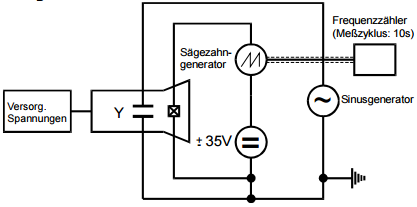
\includegraphics[height=5cm]{picture/Schaltung2}
  \caption{Aufbau eines Kathodenstrahl-Oszillographen. \cite[5]{V501}}
  \label{fig:Schaltung2}
\end{figure}

Es sollen stehende Sinuswellen auf dem Oszillographen zu erkennen sein. Dazu wird die Frequenz der Sägezahnspannung so lange verändert bis das Verhältnis $n$ zwischen der Sägezahnfrequenz und der Sinusfrequenz $n = \frac{1}{2}, 1, 2 \text{und} 3$ entspricht. Für jedes dieser Verhältnisse wird die Frequenz und die Amplitude (y-Achse) der Sinuswelle gemessen.

\subsection{Messprogram für die Ablenkung im B-Feld}
Der Versuchsaufbau besteht aus einer Helmholtzspule und einer Kathodenstrahlröhre, welche senkrecht zum Magnetfeld der Helmholtzspule ausgerichtet ist. \\
Zu Beginn wird die Nord-Süd Richtung und der Inklinationswinkel des Erdmagnetfeldes ermittelt und der Versuchsaufbau so ausgerichtet, dass die Kathodenstrahlröhre parallel zur Horizontalkomponente des Erdmagnetfeldes ist. Daraufhin wird mit Hilfe des Ablenksystems der Kathodenstrahlröhre der Leuchtfleck auf die unterste Linie gebracht. Nun wird die Stromstärke, die die Stärke des Magnetfeldes der Helmholtzspule regelt, so lange erhöht bis der Leuchtfleck auf der ersten Linie des Koordinatennetzes ist und es wird die Stromstärke notiert. Dies wird für die weiteren Linien wiederholt. \\
Im zweiten Versuchsteil wird die Helmholtzspule ausgeschaltet und der Leuchtfleck auf die mittlere Linie gebracht. Danach wird der gesamte Versuchsaufbau um 90° gedreht sodass die Elektronen in der Kathodenstrahlröhre vom Erdmagnetfeld abgelenkt werden. Sodann wird die Helmholtzspule wieder eingeschaltet und der Leuchtfleck wieder in seine Ausgangsposition gebracht. Die dafür benötigte Stromstärke und die Verschiebung des Leuchtflecks werden notiert.





















a
